%
% lie-algebren.tex -- Lie-Algebren
%
% (c) 2020 Prof Dr Andreas Müller, Hochschule Rapperswil
%
\section{Lie-Algebren
\label{buch:section:lie-algebren}}
Im vorangegangenen Abschnitt wurde gezeigt, dass alle beschriebenen
Matrizengruppen als Untermannigfaltigkeiten im $n^2$-dimensionalen
Vektorraum $M_n(\mathbb{R})$ betrachtet werden können.
Die Gruppen haben damit nicht nur die algebraische Struktur einer
Matrixgruppe, sie haben auch die geometrische Struktur einer 
Mannigfaltigkeit.
Insbesondere ist es sinnvoll, von Ableitungen zu sprechen.

Eindimensionale Untergruppen einer Gruppe können auch als Kurven
innerhalb der Gruppe angesehen werden.
In diesem Abschnitt soll gezeigt werden, wie man zu jeder eindimensionalen
Untergruppe einen Vektor in $M_n(\mathbb{R})$ finden kann derart, dass
der Vektor als Tangentialvektor an diese Kurve gelten kann.
Aus einer Abbildung zwischen der Gruppe und diesen Tagentialvektoren
erhält man dann auch eine algebraische Struktur auf diesen Tangentialvektoren,
die sogenannte Lie-Algebra.
Sie ist charakteristisch für die Gruppe.
Insbesondere werden wir sehen, wie die Gruppen $\operatorname{SO}(3)$ 
und $\operatorname{SU}(2)$ die gleich Lie-Algebra haben und dass die
Lie-Algebra von $\operatorname{SO}(3)$ mit dem Vektorprodukt in $\mathbb{R}^3$
übereinstimmt.
\index{Vektorprodukt}%

\rhead{Lie-Algebren}
%
% Die Lie-Algebra einer Matrizengruppe
%
\subsection{Lie-Algebra einer Matrizengruppe
\label{buch:section:lie-algebra-einer-matrizengruppe}}
Zu jedem Tangentialvektor $A$ im Punkt $I$ einer Matrizengruppe gibt es
eine Einparameteruntergruppe, die mit Hilfe der Exponentialfunktion
$e^{At}$ konstruiert werden kann.
Für die folgende Konstruktion arbeiten wir in der Gruppe
$\operatorname{GL}_n(\mathbb{R})$, in der jede Matrix auch ein
Tangentialvektor ist.
Wir werden daraus die Lie-Klammer ableiten und später verifizieren,
dass diese auch für die Tangentialvektoren der Gruppen
$\operatorname{SO}(n)$ oder $\operatorname{SL}_n(\mathbb{R})$ funktioniert.

\subsubsection{Lie-Klammer}
Zu zwei verschiedenen Tagentialvektoren $A\in M_n(\mathbb{R})$ und
$B\in M_n(\mathbb{R})$ gibt es zwei verschiedene Einparameteruntergruppen
$e^{At}$ und $e^{Bt}$.
Wenn die Matrizen $A$ und $B$ oder die Einparameteruntergruppen 
$e^{At}$ und $e^{Bt}$ vertauschbar sind, dann stimmen 
$e^{At}e^{Bt}$ und $e^{Bt}e^{At}$ nicht überein.
Die zugehörigen Potenzreihen sind:
\begin{align*}
e^{At}
&=
I+At + \frac{A^2t^2}{2!} + \frac{A^3t^3}{3!} + \dots
\\
e^{Bt}
&=
I+Bt + \frac{B^2t^2}{2!} + \frac{B^3t^3}{3!} + \dots
\\
e^{At}e^{Bt}
&=
\biggl(I+At + \frac{A^2t^2}{2!} + \dots\biggr)
\biggl(I+Bt + \frac{B^2t^2}{2!} + \dots\biggr)
\\
&=
I+(A+B)t + \biggl(\frac{A^2}{2!}+AB+\frac{B^2}{2!}\biggr)t^2 +\dots
\\
e^{Bt}e^{At}
&=
\biggl(I+Bt + \frac{B^2t^2}{2!} + \dots\biggr)
\biggl(I+At + \frac{A^2t^2}{2!} + \dots\biggr)
\\
&=
I+(B+A)t + \biggl(\frac{B^2}{2!}+BA+\frac{A^2}{2!}\biggr)t^2 +\dots
\intertext{%
Die beiden Kurven $e^{At}e^{Bt}$ und $e^{Bt}e^{At}$ haben zwar den gleichen
Tangentialvektor für $t=0$, sie unterscheiden
sich aber für $t>0$ und sie unterscheiden sich von der
Einparameteruntergruppe}
e^{(A+B)t}
&=
I + (A+B)t + \frac{t^2}{2}(A^2 + AB + BA + B^2) + \ldots
\intertext{von $A+B$. Für die Unterschiede finden wir}
e^{At}e^{Bt} - e^{(A+B)t}
&=
\biggl(AB-\frac{AB+BA}2\biggr)t^2
+\ldots
=
(AB-BA) \frac{t^2}{2} + \ldots
=
\phantom{-}
[A,B]\frac{t^2}{2}+\ldots
\\
e^{Bt}e^{At} - e^{(A+B)t}
&=
\biggl(BA-\frac{AB+BA}2\biggr)t^2
+\ldots,
=
(BA-AB)
\frac{t^2}{2}
+\ldots
=
-[A,B]\frac{t^2}{2}+\ldots,
\\
e^{At}e^{Bt}-e^{Bt}e^{At}
&=
(AB-BA)t^2+\ldots
=
\phantom{-}[A,B]t^2+\ldots,
\end{align*}
wobei $[A,B]=AB-BA$ abgekürzt wird.

\begin{definition}
\label{buch:gruppen:def:kommutator}
Der {\em Kommutator} zweier Matrizen $A,B\in M_n(\mathbb{R})$ ist die Matrix
$[A,B]=AB-BA$.
\index{Kommutator}%
\index{Lie-Klammer}%
\end{definition}

Der Kommutator ist bilinear und antisymmetrisch, da
\index{bilinear}%
\index{antisymmetrisch}%
\begin{align*}
[\lambda A+\mu B,C]
&=
\lambda AC+\mu BC-\lambda CA -\mu CB
=
\lambda[A,C]+\mu[B,C]
\\
[A,\lambda B+\mu C]
&=
\lambda AB + \mu AC - \lambda BA - \mu CA
=
\lambda[A,B]+\mu[A,C]
\\
[A,B]
&=
AB-BA = -(BA-AB) = -[B,A].
\end{align*}
Aus der letzten Bedingung folgt insbesodnere $[A,A]=0$

Der Kommutator $[A,B]$ misst in niedrigster Ordnung den Unterschied
zwischen den
$ e^{At} e^{Bt} $
und
$ e^{Bt} e^{At} $.
Der Kommutator der Tangentialvektoren $A$ und $B$ bildet also die
Nichtkommutativität der Matrizen $e^{At}$ und $e^{Bt}$ ab.

\subsubsection{Die Jacobi-Identität}
Der Kommutator hat die folgende zusätzliche algebraische Eigenschaft:
\begin{align*}
[A,[B,C]]
+
[B,[C,A]]
+
[C,[A,B]]
&=
[A,BC-CB]
+
[B,CA-AC]
+
[C,AB-BA]
\\
&=\phantom{+}
ABC-ACB-BCA+CBA
\\
&\phantom{=}+
BCA-BAC-CAB+ACB
\\
&\phantom{=}+
CAB-CBA-ABC+BAC
\\
&=0.
\end{align*}
Diese Eigenschaft findet man auch bei anderen Strukturen, zum Beispiel
bei Vektorfeldern, die man als Differentialoperatoren auf Funktionen 
betrachten kann.
Man kann dann einen Kommutator $[X,Y]$ für zwei Vektorfelder
$X$ und $Y$ definieren.
Dieser Kommutator von Vektorfeldern erfüllt ebenfalls die gleiche
Identität.

\begin{definition}
\label{buch:gruppen:def:jacobi}
Ein bilineares Produkt $[\;,\;]\colon V\times V\to V$ auf dem Vektorraum
erfüllt die {\em Jacobi-Identität}, wenn 
\index{Jacobi-Identität}%
\[
[u,[v,w]] + [v,[w,u]] + [w,[u,v]]=0
\]
ist für beliebige Vektoren $u,v,w\in V$.
\end{definition}

\subsubsection{Lie-Algebra}
Die Tangentialvektoren einer Lie-Gruppe tragen also mit dem Kommutator
eine zusätzliche Struktur, nämlich die Struktur einer Lie-Algebra.

\begin{definition}
Ein Vektorraum $V$ mit einem bilinearen, Produkt
\[
[\;,\;]\colon V\times V \to V : (u,v) \mapsto [u,v],
\]
welches zusätzlich die Jacobi-Identität~\ref{buch:gruppen:def:jacobi}
erfüllt, heisst eine {\em Lie-Algebra}.
\index{Lie-Algebra}%
\end{definition}

Die Lie-Algebra einer Lie-Gruppe $G$ wird mit $LG$ bezeichnet.
$LG$ besteht aus den Tangentialvektoren im Punkt $I$.
Die {\em Exponentialabbildung} $\exp\colon LG\to G:A\mapsto e^A$
\index{Exponentialabbildung}%
ist eine differenzierbare Abbildung von $LG$ in die Gruppe $G$.
Insbesondere kann die Inverse der Exponentialabbildung als eine
Karte in einer Umgebung von $I$ verwendet werden.

Für die Lie-Algebren der Matrizengruppen, die früher definiert worden
sind, verwenden wir die Notationskonvention, dass der Name der
Lie-Algebra der mit kleinen Buchstaben geschrieben Name der Lie-Gruppe ist.
Die Lie-Algebra von $\operatorname{SO}(n)$ ist also
$L\operatorname{SO}(n) = \operatorname{so}(n)$,
\index{so(n)@$\operatorname{so}(n)$}%
die Lie-Algebra von $\operatorname{SL}_n(\mathbb{R})$ ist
$L\operatorname{SL}_n(\mathbb{R})=\operatorname{sl}_n(\mathbb{R})$.
\index{sln(r)@$\operatorname{sl}_n(\mathbb{R})$}%

%
% Die Lie-Algebra von SO(3)
%
\subsection{Die Lie-Algebra von $\operatorname{SO}(3)$
\label{buch:subsection:die-lie-algebra-von-so3}}
Zur Gruppe $\operatorname{SO}(3)$ der Drehmatrizen gehört die Lie-Algebra
$\operatorname{so}(3)$ der antisymmetrischen $3\times 3$-Matrizen.
Solche Matrizen haben die Form
\[
\Omega
=
\begin{pmatrix}
    0    &-\omega_3& \omega_2\\
 \omega_3&   0     &-\omega_1\\
-\omega_2& \omega_1&    0
\end{pmatrix}
\]
Die antisymmetrischen Matrizen
\[
\Omega_{23}
=
\begin{pmatrix} 0&0&0\\0&0&-1\\0&1&0\end{pmatrix},
\quad
\Omega_{31}
=
\begin{pmatrix} 0&0&1\\0&0&0\\-1&0&0\end{pmatrix},
\quad
\Omega_{12}
=
\begin{pmatrix} 0&1&0\\-1&0&0\\0&0&0\end{pmatrix}
\]
bilden eine Basis für $\operatorname{so}(3)$, man kann
\[
\Omega
=
\omega_1\Omega_{23}
+
\omega_2\Omega_{31}
+
\omega_3\Omega_{12}
\]
schreiben.
Der Vektorraum $\operatorname{so}(3)$ ist also dreidimensional.

Die Kommutatoren der Basisvektoren sind
\begin{equation}
\setlength\arraycolsep{4pt}
\begin{aligned}
[\Omega_{23},\Omega_{31}]
&=
\begin{pmatrix}
0&-1&0\\
1&0&0\\
0&0&0
\end{pmatrix}
=
\Omega_{12},
%\\
&
[\Omega_{31},\Omega_{12}]
&=
\begin{pmatrix}
0&0&0\\
0&0&-1\\
0&1&0
\end{pmatrix}
=
\Omega_{23},
%\\
&
[\Omega_{12},\Omega_{23}]
&=
\begin{pmatrix}
0&0&1\\
0&0&0\\
-1&0&0
\end{pmatrix}
=
\Omega_{31},
\end{aligned}
\label{buch:gruppen:eqn:so3-kommutatoren}
\end{equation}
wie man durch direkte Rechnung bestätigt.
Diese Regeln stimmen mit den Vektorprodukten der Standardbasisvektoren
in $\mathbb{R}^3$ überein.

\begin{figure}
\centering
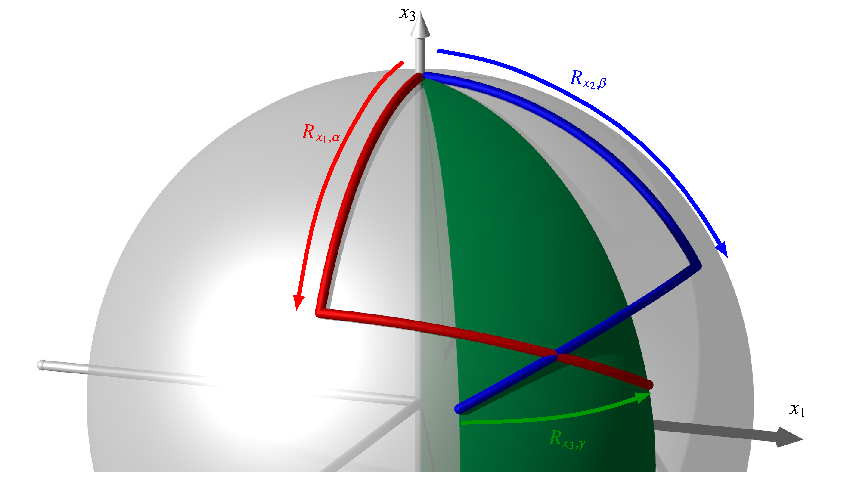
\includegraphics{chapters/60-gruppen/images/nichtkomm.pdf}
\caption{Der Kommutator zweier Drehungen um die $x_1$ und $x_2$
Achse ist eine Drehung um die $x_3$-Achse.
\label{buch:lie:fig:kommutator}}
\end{figure}
Abbildung~\ref{buch:lie:fig:kommutator} illustriert, wie der
Kommutator die Nichtkommutativität der Gruppe $\operatorname{SO}(3)$
wiedergibt.
Die Matrix $\Omega_{23}$ erzeugt eine Drehung $R_{x_1,\alpha}$
um die $x_1$-Achse,
die Matrix $\Omega_{31}$ eine Drehung $R_{x_2,\beta}$ um die $x_2$ Achse.
Der Kommutator $[\Omega_{23},\Omega_{31}]=\Omega_{12}$ beschreibt in
niedrigster Ordnung den Unterschied, der entsteht, wenn man die
beiden Drehungen in verschiedenen Reihenfolgen ausführt.
Dies ist eine Drehung $R_{x_3,\gamma}$ um die $x_3$-Achse.

Aus der Rodrigues-Formel~\ref{buch:lie:eqn:rodrigues} wissen wir
bereits, dass die Ableitung der Drehung das Vektorprodukt
$\vec{\omega}\times\vec{x}$ ist.
Dieses kann jedoch auch als
$\Omega\vec{x} = \vec{\omega}\times\vec{x}$
ausgedrückt werden.

Die Wirkung von $I+t\Omega$ auf einem Vektor $\vec{x}$ ist
\[
(I+t\Omega)
\begin{pmatrix}x_1\\x_2\\x_3\end{pmatrix}
=
\begin{pmatrix}
    1     &-t\omega_3& t\omega_2\\
 t\omega_3&   1      &-t\omega_1\\
-t\omega_2& t\omega_1&    1
\end{pmatrix}
\begin{pmatrix}x_1\\x_2\\x_3\end{pmatrix}
=
\begin{pmatrix}
x_1+t(-\omega_3x_2+\omega_2x_3)\\
x_2+t( \omega_3x_1-\omega_1x_3)\\
x_3+t(-\omega_2x_1+\omega_1x_2)
\end{pmatrix}
=
\vec{x}+ t\begin{pmatrix}\omega_1\\\omega_2\\\omega_3\end{pmatrix}\times x
=
\vec{x}+ t\vec{\omega}\times \vec{x}.
\]
Die Matrix $\Omega$ ist als die infinitesimale Version einer Drehung
um die Achse $\omega$.

Wir können die Analogie zwischen Matrizen in $\operatorname{so}(3)$ und
Vektoren in $\mathbb R^3$ noch etwas weiter treiben. Zu jedem Vektor
in $\mathbb R^3$ konstruieren wir eine Matrix in $\operatorname{so}(3)$
mit Hilfe der Abbildung
\[
\mathbb R^3\to\operatorname{so}(3)
:
\begin{pmatrix}v_1\\v_2\\v_3\end{pmatrix}
\mapsto
\begin{pmatrix}
  0 &-v_3& v_2\\
 v_3&  0 &-v_1\\
-v_2& v_1&  0
\end{pmatrix}.
\]
Der Kommutator von zwei so aus Vektoren $\vec u$ und $\vec v$
konstruierten Matrizen $U$ und $V$ ist:
\begin{align*}
[U,V]
&=
UV-VU
\\
&=
\begin{pmatrix}
  0 &-u_3& u_2\\
 u_3&  0 &-u_1\\
-u_2& u_1&  0
\end{pmatrix}
\begin{pmatrix}
  0 &-v_3& v_2\\
 v_3&  0 &-v_1\\
-v_2& v_1&  0
\end{pmatrix}
-
\begin{pmatrix}
  0 &-v_3& v_2\\
 v_3&  0 &-v_1\\
-v_2& v_1&  0
\end{pmatrix}
\begin{pmatrix}
  0 &-u_3& u_2\\
 u_3&  0 &-u_1\\
-u_2& u_1&  0
\end{pmatrix}
\\
&=
\begin{pmatrix}
-u_3v_3-u_2v_2 + u_3v_3 + u_2v_2
        & u_2v_1 - u_1v_2
                & u_3v_1 - u_1v_3
\\
u_1v_2 - u_2v_1
        & -u_3v_3-u_1v_1 + u_3v_3+u_1v_1
                & u_3v_2 - u_2v_3
\\
u_1v_3 - u_3v_1
        & u_2v_3 - u_3v_2
                &-u_2v_2-u_1v_1+ u_2v_2+u_1v_1
\end{pmatrix}
\\
&=
\begin{pmatrix}
0
        &-(u_1v_2 - u_2v_1)
                &u_3v_1-u_1v_3
\\
u_1v_2 - u_2v_1
        & 0
                &-(u_2v_3 - u_3v_2)
\\
-(u_3v_1 - u_1v_3)
        &   u_3v_2 - u_2v_3
                & 0
\end{pmatrix}.
\end{align*}
Die Matrix $[U,V]$ gehört zum Vektor $\vec u\times\vec v$.
Damit können wir aus der Jacobi-Identität jetzt folgern, dass
\[
\vec u\times(\vec v\times w)
+
\vec v\times(\vec w\times u)
+
\vec w\times(\vec u\times v)
=0
\]
für drei beliebige Vektoren $\vec u$, $\vec v$ und $\vec w$ ist.
Dies bedeutet, dass der dreidimensionale Vektorraum $\mathbb R^3$
mit dem Vektorprodukt zu einer Lie-Algebra wird.
In der Tat verwenden einige Lehrbücher statt der vertrauten Notation
$\vec u\times \vec v$ für das Vektorprodukt die aus der Theorie der
Lie-Algebren entlehnte Notation $[\vec u,\vec v]$, zum Beispiel
auch das Lehrbuch der Theoretischen Physik \cite{skript:landaulifschitz1}
von Landau und Lifschitz.

Die Lie-Algebren sind vollständig klassifiziert worden, es gibt
keine nicht trivialen zweidimensionalen Lie-Algebren.
Unser dreidimensionaler Raum ist also auch in dieser Hinsicht speziell:
es ist der kleinste Vektorraum, in dem eine nichttriviale Lie-Algebra-Struktur
möglich ist.

\subsection{Die Lie-Algebra von $\operatorname{SL}_n(\mathbb{R})$}
Die Lie-Algebra von $\operatorname{SL}_n(\mathbb{R})$ besteht aus den
spurlosen Matrizen in $M_n(\mathbb{R})$.
Der Kommutator solcher Matrizen erfüllt
\[
\operatorname{Spur}([A,B])
=
\operatorname{Spur}(AB-BA)
=
\operatorname{Spur}(AB)-\operatorname{Spur}(BA)
=
0,
\]
somit ist 
\[
\operatorname{sl}_n(\mathbb{R})
=
\{
A\in M_n(\mathbb{R}) \mid \operatorname{Spur}(A)=0
\}
\]
mit dem Kommutator von Matrizen als Lie-Klammer eine Lie-Algebra.

%
% Die Lie-Algebra von U(n)
%
\subsection{Die Lie-Algebra von $\operatorname{U}(n)$}
Die Lie-Gruppe
\[
U(n)
=
\{
A\in M_n(\mathbb{C})
\mid
AA^*=I
\}
\]
\index{unitäre Gruppe}%
\index{Gruppe, unitär}%
\index{U(n)@$\operatorname{U}(n)$}%
heisst die unitäre Gruppe, sie besteht aus den Matrizen, die
das sesquilineare Standardskalarprodukt auf dem komplexen
Vektorraum $\mathbb{C}^n$ invariant lassen.
Sei $\gamma(t)$ eine differenzierbare Kurve in $\operatorname{U}(n)$
derart, dass $\gamma(0)=I$.
Die Ableitung der Identität $AA^*=I$ führt dann auf 
\begin{equation*}
0
=
\frac{d}{dt}
\gamma(t)\gamma(t)^*
\bigg|_{t=0}
=
\dot{\gamma}(0)\gamma(0)^*
+
\gamma(0)\dot{\gamma}(0)^*
=
\dot{\gamma}(0)
+
\dot{\gamma}(0)^*
\quad\Rightarrow\quad
\dot{\gamma}(0)=-\dot{\gamma}(0)^*
\quad\Rightarrow\quad
A=-A^*
\end{equation*}
Die Lie-Algebra $\operatorname{u}(n)$ besteht daher aus den antihermiteschen
Matrizen.
\index{u(n)@$\operatorname{u}(n)$}%

Wir sollten noch verifizieren, dass der Kommutator zweier antihermiteschen
Matrizen wieder antihermitesch ist:
\index{antihermitesch}%
\begin{align*}
[A,B]^*
&=
(AB-BA)^*
=
B^*A^*-A^*B^*
=
BA - AB
=
-[B,A].
\end{align*}

Eine antihermitesche Matrix erfüllt $a_{i\!j}=-\overline{a}_{ji}$,
für die Diagonalelemente folgt daher $a_{ii} = -\overline{a}_{ii}$
oder $\overline{a}_{ii}=-a_{ii}$.
Der Realteil von $a_{ii}$ ist
\[
\Re a_{ii}
=
\frac{a_{ii}+\overline{a}_{ii}}2
=
0,
\]
die Diagonalelemente einer antihermiteschen Matrix sind daher rein
imaginär.


%
% Die Lie-Algebra SU(2)
%
\subsection{Die Lie-Algebra von $\operatorname{SU}(2)$}
Die Lie-Algebra $\operatorname{su}(n)$ besteht aus den
spurlosen antihermiteschen $2\times 2$-Matrizen.
\index{su(n)@$\operatorname{su}(n)$}%
Sie erfüllen daher die folgenden Bedingungen:
\[
A=\begin{pmatrix}a&b\\c&d\end{pmatrix}
\qquad
\text{mit}
\qquad
\left\{
\begin{aligned}
a+d&=0&&\Rightarrow& a=is = -d
\\
b^*&=-c
\end{aligned}
\right.
\]
Damit hat $A$ die Form
\begin{align*}
A=\begin{pmatrix}
is&u+iv\\
-u+iv&-is
\end{pmatrix}
&=
s
\begin{pmatrix}
i&0\\
0&-i
\end{pmatrix}
+
u
\begin{pmatrix}
 0&1\\
-1&0
\end{pmatrix}
+
v
\begin{pmatrix}
0&i\\
i&0
\end{pmatrix}
\\
&=
iv\underbrace{\begin{pmatrix}0&1\\1&0\end{pmatrix}}_{\displaystyle=\sigma_1}
+
iu\underbrace{\begin{pmatrix}0&-i\\i&0\end{pmatrix}}_{\displaystyle=\sigma_2}
+
is\underbrace{\begin{pmatrix}1&0\\0&-1\end{pmatrix}}_{\displaystyle=\sigma_3}
\end{align*}
Diese Matrizen heissen die {\em Pauli-Matrizen}, sie haben die Kommutatoren
\index{Pauli-Matriizen}%
\begin{align*}
[\sigma_1,\sigma_2]
&=
\begin{pmatrix}0&1\\1&0\end{pmatrix}
\begin{pmatrix}0&-i\\i&0\end{pmatrix}
-
\begin{pmatrix}0&-i\\i&0\end{pmatrix}
\begin{pmatrix}0&1\\1&0\end{pmatrix}
=
2\begin{pmatrix}i&0\\0&-i \end{pmatrix}
=
2i\sigma_3,
\\
[\sigma_2,\sigma_3]
&=
\begin{pmatrix}0&-i\\i&0\end{pmatrix}
\begin{pmatrix}1&0\\0&-1\end{pmatrix}
-
\begin{pmatrix}1&0\\0&-1\end{pmatrix}
\begin{pmatrix}0&-i\\i&0\end{pmatrix}
=
2
\begin{pmatrix}0&i\\i&0\end{pmatrix}
=
2i\sigma_1.
\\
[\sigma_1,\sigma_3]
&=
\begin{pmatrix}0&1\\1&0\end{pmatrix}
\begin{pmatrix}1&0\\0&-1\end{pmatrix}
-
\begin{pmatrix}1&0\\0&-1\end{pmatrix}
\begin{pmatrix}0&1\\1&0\end{pmatrix}
=
2i
\begin{pmatrix}0&-1\\1&0\end{pmatrix}
=
2i\sigma_2,
\end{align*}
Bis auf eine Skalierung stimmt dies überein mit den Kommutatorprodukten
der Matrizen $\Omega_{23}$, $\Omega_{31}$ und $\Omega_{12}$
in \eqref{buch:gruppen:eqn:so3-kommutatoren}.
Die Matrizen $-\frac12i\sigma_j$ haben die Kommutatorprodukte
\begin{align*}
\bigl[-{\textstyle\frac12}i\sigma_1,-{\textstyle\frac12}i\sigma_2\bigr]
&=
-{\textstyle\frac14}[\sigma_1,\sigma_2]
=
-{\textstyle\frac14}\cdot 2i\sigma_3
=
-{\textstyle\frac12}i\sigma_3
\\
\bigl[-{\textstyle\frac12}i\sigma_2,-{\textstyle\frac12}i\sigma_3\bigr]
&=
-{\textstyle\frac14}[\sigma_2,\sigma_3]
=
-{\textstyle\frac14}\cdot 2i\sigma_1
=
-{\textstyle\frac12}i\sigma_1
\\
\bigl[-{\textstyle\frac12}i\sigma_3,-{\textstyle\frac12}i\sigma_1\bigr]
&=
-{\textstyle\frac14}[\sigma_3,\sigma_1]
=
-{\textstyle\frac14}\cdot 2i\sigma_2
=
-{\textstyle\frac12}i\sigma_2.
\end{align*}
Die lineare Abbildung, die
\begin{align*}
\Omega_{23}&\mapsto -{\textstyle\frac12}i\sigma_1\\
\Omega_{31}&\mapsto -{\textstyle\frac12}i\sigma_2\\
\Omega_{12}&\mapsto -{\textstyle\frac12}i\sigma_3
\end{align*}
abbildet, ist daher ein Isomorphismus der Lie-Algebra $\operatorname{so}(3)$
auf die Lie-Algebra $\operatorname{su}(2)$.
Die Lie-Gruppen $\operatorname{SO}(3)$ und $\operatorname{SU}(2)$
haben also die gleiche Lie-Algebra.

Tatsächlich kann man Hilfe von Quaternionen die Matrix $\operatorname{SU}(2)$
als Einheitsquaternionen beschreiben und damit eine Darstellung der
Drehmatrizen in $\operatorname{SO}(3)$ finden.
Dies wird in Kapitel~\ref{chapter:clifford} dargestellt.





